\chapter{Svojstvene vrijednosti i svojstvene funkcije Laplaceovog operatora}
\label{chp:Dirichlet_Laplacian}

Prije same definicije svojstvenih vrijednosti i svojstvenih funkcija Laplaceovog operatora, navest ćemo neke njihove primjene i važnosti. Ukratko, to su realne vrijednosti i realne funkcije pridružene nekom skupu točaka (domeni svojstvenih funkcija) koje ovise o tom skupu točaka.

\par

D.\ Benguria u~\cite{bib:Benguria_Dirichlet_eigenvalue} objašnjava da su se svojstvene vrijednosti i svojstvene funkcije Laplaceovog operatora počele proučavati istraživanjem vibracija napete membrane. U istom je izvoru navedeno da su prirodne frekvencije tijela (frekvencije kojima to tijelo \emph{prirodno} vibrira nakon postavljanja u nestabilan položaj) recipročne korijenima svojstvenih vrijednosti, dok je u~\cite{bib:COMSOL18} pak prikazano da se vibrirajuće tijelo iskrivljuje u obliku svojstvenih funkcija. U potonjem je izvoru dodatno objašnjeno da su vibracije u višim prirodnim frekvencijama sklonije prigušenju, štoviše, njihov će udio od početka vibriranja biti zanemariv. Osim primjene u analizi vibrirajućih tijela, Reuter i dr.\ u~\cite{bib:Reuter09} pokazuju da se mnoga svojstva oblika domene mogu zaključiti iz njezinih svojstvenih vrijednosti, a praktično dokazuju da je pritom dovoljno proučavati opet samo konačni broj najnižih svojstvenih vrijednosti.

\par

Predočimo fenomen prigušenosti i zastupljenosti prirodnih frekvencija spomenut u prethodnom odlomku realnim primjerom sviranja žičanog instrumenta poput violine ili gitare gdje je vibrirajuće tijelo žica. Trznemo li žicu, ona će dominantno vibrirati po svojoj prvoj prirodnoj frekvenciji (jedan \emph{luk}---u terminima funkcija, jedan lokalni ekstrem) i to je, zapravo, onaj ton koji žica proizvodi. Tek flažoletima možemo potencirati vibriranje po nekoj višoj prirodnoj frekvenciji ($ \numprint{2} $, $ \numprint{3} $ ili više \emph{lukova} odnosno lokalnih ekstrema). Međutim, sviranjem flažoleta ton će se brže utišati i žica će na kraju ipak dominantno vibrirati po svojoj prvoj prirodnoj frekvenciji.

\par

Što se tiče stvarne definicije, Dirichletove svojstvene vrijednosti i svojstvene funkcije D.\ Benguria definirao je u~\cite{bib:Benguria_Dirichlet_eigenvalue} slično kao što je definirano u definiciji~\ref{def:Laplacian_eigen}, samo što u definiciji~\ref{def:Laplacian_eigen} koristimo drugačiju terminologiju\footnote{U literaturi se pojavljuju različiti termini: D.\ Benguria u~\cite{bib:Benguria_Dirichlet_eigenvalue} koristi termin \emph{Dirichletova svojstvena vrijednost}, Laugesen i Siudeja u~\cite{bib:Laugesen10} koriste termine \emph{Dirichletova svojstvena vrijednost Laplaceovog operatora} i \emph{svojstvena vrijednost Dirichletovog Laplaceovog operatora}, Reuter i dr.\ u~\cite{bib:Reuter09} promatraju generalizirani problem koristeći termine \emph{svojstvena vrijednost Laplace-Beltramijevog operatora}, \emph{svojstvena vrijednost \emph{volumetričnog} Laplaceovog operatora} i \emph{svojstvena vrijednost Laplaceovog operatora}\ldots{} Eksplicitno naglašavanje da se radi o \emph{Dirichletovom Laplaceovom operatoru} ili o \emph{Dirichletovim svojstvenim vrijednostima} znači da se uzima nul-rubni uvjet kao u~\eqref{eq:Dirichlet_Laplacian_problem}, kakav se u ostatku rada samo i razmatra.} i postavljamo dodatna ograničenja na domenu, svojstvene vrijednosti i svojstvene funkcije.

\par

\begin{definition} \label{def:Laplacian_eigen}
    Neka je $ n \in \positives{\naturals} $. Neka je $ \Omega \subseteq \reals^{n} $ neprazan, ograničen i otvoren takav da je $ \boundary \Omega $ po dijelovima gladak. Za $ \lambda \in \reals $ kažemo da je \defined{svojstvena vrijednost Laplaceovog operatora na skupu $ \Omega $} ako postoji neprekidna funkcija $ u \colon \closure{\Omega} \to \reals $ dvaput diferencijabilna na $ \Omega $ koja nije konstantna tako da vrijedi
    \begin{equation} \label{eq:Dirichlet_Laplacian_problem}
        \begin{eqsystem}
            {- {\Laplacian u}} & = \lambda u \text{,} & \text{na} \ \Omega \text{,} \\
            u & = \numprint{0} \text{,} & \text{na} \ \boundary \Omega
        \end{eqsystem}
    \end{equation}
    i u tom slučaju funkciju $ u $ zovemo \defined{svojstvena funkcija Laplaceovog operatora na skupu $ \Omega $}. Svojstvene vrijednosti i svojstvene funkcije Laplaceovog operatora na skupu $ \Omega $ koje u paru zadovoljavaju~\eqref{eq:Dirichlet_Laplacian_problem} zovemo \defined{(međusobno) pripadnima}.

    \par

    \defined{Kratnost svojstvene vrijednosti Laplaceovog operatora na skupu $ \Omega $} dimenzija je vektorskog potprostora njoj pripadnih svojstvenih funkcija (kada bismo prihvaćali i konstantnu nul-funkciju kao pripadnu svojstvenu funkciju).
\end{definition}

\par

Svojstvene vrijednosti i svojstvene funkcije iz definicije~\ref{def:Laplacian_eigen} u nekim su slučajevima vrlo \emph{jednostavne} vrijednosti i funkcije. Na primjer, za skup $ \Omega = \intervaloo{\numprint{0}}{\pi} \subseteq \reals $ jedna svojstvena vrijednost i pripadna svojstvena funkcija su $ \lambda = \numprint{1} $ i $ u = \restrict{{\sin}}{\intervalcc{\numprint{0}}{\pi}} $. Na nekim \emph{kompliciranijim} domenama svojstvene vrijednosti i svojstvene funkcije možda nije moguće egzaktno izraziti u zatvorenoj formi (ili bi barem taj izraz u nekoj praktičnoj svrsi bio nepotrebno \emph{ružan}, \emph{dugačak} ili \emph{kompliciran}), ali moguće ih je numerički aproksimirati.

\par

U definiciji~\ref{def:Laplacian_eigen} spominje se vektorski potprostor svojstvene vrijednosti Laplaceovog operatora. Naravno, zbog linearnosti diferencijala za svaku svojstvenu vrijednost postoji cijeli vektorski potprostor pripadnih svojstvenih funkcija.

\par

Za svojstvene vrijednosti Laplaceovog operatora, nadalje, D.\ Benguria u~\cite{bib:Benguria_Dirichlet_eigenvalue} iskazuje da vrijedi
\begin{equation*}
    \numprint{0} < \lambda_{\numprint{1}} \leq \lambda_{\numprint{2}} \leq \cdots \leq \lambda_{k} \leq \cdots \uparrow {+ \infty} \text{.}
\end{equation*}
Drugim riječima,
\begin{enumerate}
    \item \label{itm:Laplace_eigenvalue_smallest} postoji najmanja svojstvena vrijednost $ \lambda_{\numprint{1}} $ i ona je strogo pozitivna,
    \item \label{itm:Laplace_eigenvalue_countability} svojstvenih vrijednosti je prebrojivo beskonačno mnogo,
    \item \label{itm:Laplace_eigenvalue_no_accumulation} niz svojstvenih vrijednosti nema gomilište---posebno, neograničen je odozgo.
\end{enumerate}

\par

\begin{definition} \label{def:spectrum}
    Neka je $ n \in \positives{\naturals} $. Neka je $ \Omega \subseteq \reals^{n} $ neprazan, ograničen i otvoren takav da je $ \boundary \Omega $ po dijelovima gladak. Rastući niz svih svojstvenih vrijednosti Laplaceovog operatora na skupu $ \Omega $ tako da se svaka svojstvena vrijednost u nizu pojavljuje onoliko puta kolika joj je kratnost zovemo \defined{spektar skupa $ \Omega $} i označavamo sa \defined{$ \spectrum \left( \Omega \right) $}.
\end{definition}

\par

\section{Pojednostavljenje problema računanja spektra normalizacijom domena}
\label{sec:spectrum_simplification_domain_normalisation}

Problem računanja spektra moguće je donekle pojednostaviti s obzirom na neka njegova svojstva. Konkretno, domenu je moguće \emph{normalizirati} i/ili aproksimirati nekom drugom domenom i na taj način računati i/ili aproksimirati njezin spektar.

\par

\begin{definition} \label{def:similarity}
    Neka je $ n \in \positives{\naturals} $. Za skupove $ S , T \subseteq \reals^{n} $ kažemo da \defined{je skup $ T $ sličan skupu $ S $}, što označavamo s \defined{$ T \sim S $}, ako postoje afina izometrija $ \varphi \colon \reals^{n} \to \reals^{n} $ i skalar $ \alpha > \numprint{0} $ takvi da je
    \begin{equation}
        T = \alpha \RangeSet{\varphi}{S}
    \end{equation}
    i u tom slučaju funkciju $ \alpha \varphi $ zovemo \defined{sličnost (skupa $ T $ sa skupom $ S $)}.
\end{definition}

\par

\begin{remark} \label{rem:similarity_symmetry}
    Relacija sličnosti iz definicije~\ref{def:similarity} relacija je ekvivalencije. Stoga ćemo koristiti i neusmjerene izraze poput \emph{skupovi $ S $ i $ T $ su slični}, što znači da vrijedi $ S \sim T $ odnosno $ T \sim S $. Isto tako, ako su u nekoj familiji skupova svi skupovi u parovima slični, onda ćemo reći da \emph{su svi skupovi (u toj familiji skupova) slični}.
\end{remark}

\par

\begin{theorem} \label{thm:Laplacian_eigenvalue_similar_domains}
    Neka je $ n \in \positives{\naturals} $ proizvoljan. Neka su $ \Omega_{\numprint{1}} , \Omega_{\numprint{2}} \subseteq \reals^{n} $, $ \Omega_{\numprint{1}} , \Omega_{\numprint{2}} \neq \emptyset $, proizvoljni ograničeni i otvoreni takvi da su $ \boundary \Omega_{\numprint{1}} , \boundary \Omega_{\numprint{2}} $ po dijelovima glatki. Ako je $ \Omega_{\numprint{1}} \sim \Omega_{\numprint{2}} $ i ako je $ \alpha \varphi \colon \reals^{n} \to \reals^{n} $ sličnost skupa $ \Omega_{\numprint{2}} $ sa skupom $ \Omega_{\numprint{1}} $ za neku izometriju $ \varphi \colon \reals^{n} \to \reals^{n} $ i neki skalar $ \alpha > \numprint{0} $, onda za svaku svojstvenu vrijednost $ \lambda > \numprint{0} $ Laplaceovog operatora na skupu $ \Omega_{\numprint{2}} $ i za svaku njoj pripadnu svojstvenu funkciju $ u \colon \closure{\Omega_{\numprint{2}}} \to \reals $ je $ \alpha^{\numprint{2}} \lambda > \numprint{0} $ svojstvena vrijednost Laplaceovog operatora na skupu $ \Omega_{\numprint{1}} $ s pripadnom svojstvenom funkcijom $ \left( u \compose \alpha \varphi \right) \colon \closure{\Omega_{\numprint{1}}} \to \reals $.
\end{theorem}

\par

\begin{proof}
    Neka je $ n \in \positives{\naturals} $ proizvoljan. Neka su $ \Omega_{\numprint{1}} , \Omega_{\numprint{2}} \subseteq \reals^{n} $, $ \Omega_{\numprint{1}} , \Omega_{\numprint{2}} \neq \emptyset $, proizvoljni ograničeni i otvoreni takvi da su $ \boundary \Omega_{\numprint{1}} , \boundary \Omega_{\numprint{2}} $ po dijelovima glatki.

    \par

    Pretpostavimo da je $ \Omega_{\numprint{1}} \sim \Omega_{\numprint{2}} $. Označimo izometriju $ \varphi \colon \reals^{n} \to \reals^{n} $ i skalar $ \alpha > \numprint{0} $ tako da je $ \alpha \varphi $ sličnost skupa $ \Omega_{\numprint{2}} $ sa skupom $ \Omega_{\numprint{1}} $. Označimo $ \asmatrix{A} \in \MatrixAlgebra{\reals}{n} $ i $ \asvector{b} \in \reals^{n} $ tako da za svaki $ x \in \reals^{n} $ vrijedi $ \varphi \left( x \right) = \asmatrix{A} \asvector{x} + \asvector{b} $ u kanonskoj bazi. Budući da je $ \varphi $ izometrija, matrica $ \asmatrix{A} $ je ortogonalna, to jest, vrijedi $ \asmatrix{A} \asmatrix{A}^{\transponent} = \asmatrix{A}^{\transponent} \asmatrix{A} = \asmatrix{I} $.

    \par

    Neka je $ \lambda > \numprint{0} $ proizvoljna svojstvena vrijednost Laplaceovog operatora na skupu $ \Omega_{\numprint{2}} $ i neka je $ u \in \colon \closure{\Omega_{\numprint{2}}} \to \reals $ proizvoljna njoj pripadna svojstvena funkcija. Očito je domena funkcije $ u \compose \alpha \varphi $ skup $ \closure{\Omega_{\numprint{1}}} $, a kodomena $ \reals $. Primijetimo i da je, budući da je $ \alpha \varphi \in \Continuous{\reals^{n}}{\reals^{n}}{{+ \infty}} $, i $ u \compose \alpha \varphi $ neprekidna na $ \closure{\Omega_{\numprint{1}}} $ i dvaput diferencijabilna na $ \Omega_{\numprint{1}} $. Nadalje, po definiciji~\ref{def:Laplacian_eigen}, za $ \lambda $ i $ u $ vrijedi sustav jednadžbi~\eqref{eq:Dirichlet_Laplacian_problem} na $ \closure{\Omega_{\numprint{2}}} $, a, kako je $ \boundary \Omega_{\numprint{2}} = \RangeSet{\alpha \varphi}{\boundary \Omega_{\numprint{1}}} $, vrijedi i $ \restrict{\left( u \compose \alpha \varphi \right)}{\boundary \Omega_{\numprint{1}}} \equiv \numprint{0} $. Također, postoji $ x \in \Omega_{\numprint{1}} $ takav da je $ \left( u \compose \alpha \varphi \right) \left( x \right) \neq \numprint{0} $ jer $ u $ nije konstantna nul-funkcija ($ u \compose \alpha \varphi $ poprima vrijednost različitu od $ \numprint{0} $ u onoj točki $ x \in \Omega_{\numprint{1}} $ koja se preslikava u neku točku $ y \in \Omega_{\numprint{2}} $ u kojoj funkcija $ u $ poprima vrijednost različitu od $ \numprint{0} $).

    \par

    Neka je sada $ x \in \Omega_{\numprint{1}} $ proizvoljna točka i označimo $ \asvector{x} = \left( x_{\numprint{1}} , x_{\numprint{2}} , \dotsc , x_{n} \right) \in \reals^{n}  $ u kanonskoj bazi. Označimo $ y = \alpha \varphi \left( x \right) \in \Omega_{\numprint{2}} $ i $ \asvector{y} = \alpha \left( \asmatrix{A} \asvector{x} + \asvector{b} \right) = \left( y_{\numprint{1}} , y_{\numprint{2}} , \dotsc , y_{n} \right) \in \reals^{n} $ u kanonskoj bazi. Budući da su $ \Omega_{\numprint{1}} $ i $ \Omega_{\numprint{2}} $ otvoreni, vrijedi $ x \notin \boundary \Omega_{\numprint{1}} $ i $ y \notin \boundary \Omega_{\numprint{2}} $. Izračunajmo ($ \Laplacian_{x} $ označava \emph{standardni} Laplaceov operator; kasnije će u dokazu $ \Laplacian_{y} $ označavati sumu drugih parcijalnih derivacija po komponentama vrijednosti funkcije $ \alpha \varphi $)
    \begin{equation*}
        \begin{split}
            \Laplacian_{x} \left( u \compose \alpha \varphi \right) \left( x \right) & = \sum_{i = \numprint{1}}^{n} \PartialDerivativeSub{x}{i}{\numprint{2}} \left( u \compose \alpha \varphi \right) \left( x \right) = \\
            & = \sum_{i = \numprint{1}}^{n} \partialderivative{x_{i}} \partialderivative{x_{i}} \left( u \compose \alpha \varphi \right) \left( x \right) = \\
            & = \sum_{i = \numprint{1}}^{n} \partialderivative{x_{i}} \left( \sum_{j = \numprint{1}}^{n} \partialderivative{y_{j}} u \left( y \right) \partialderivative{x_{i}} y_{j} \right) \text{.}
        \end{split}
    \end{equation*}
    Iskoristimo činjenicu da je $ \partialderivative{x_{i}} y_{j} = \partialderivative{x_{i}} \alpha \left( \dotproduct{\asvector{a}_{j , {\cdot}}}{\asvector{x}} + b_{j} \right) = \partialderivative{x_{i}} \alpha \left( \sum_{k = \numprint{1}}^{n} a_{j k} x_{k} + b_{j} \right) = \alpha a_{j i} $, gdje $ \asvector{a}_{j , {\cdot}} \in \reals^{n} $ označava $ j $-ti redak matrice $ \asmatrix{A} $ kao vektor (dakle, vektor-stupac zapravo), $ b_{j} \in \reals $ označava $ j $-tu koordinatu vektora $ \asvector{b} $ i $ a_{j k} \in \reals $ označava element matrice $ \asmatrix{A} $ u $ j $-tom retku i $ k $-tom stupcu za svaki izbor indeksa $ j , k \in \left\{ \numprint{1} , \numprint{2} , \dotsc , n \right\} $ (ovu notaciju koristit ćemo i u ostatku dokaza). Slijedi
    \begin{multline*}
        \sum_{i = \numprint{1}}^{n} \partialderivative{x_{i}} \left( \sum_{j = \numprint{1}}^{n} \partialderivative{y_{j}} u \left( y \right) \partialderivative{x_{i}} y_{j} \right) = \sum_{i = \numprint{1}}^{n} \partialderivative{x_{i}} \left( \sum_{j = \numprint{1}}^{n} \alpha a_{j i} \partialderivative{y_{j}} u \left( y \right) \right) = \\
        = \alpha \left( \sum_{i = \numprint{1}}^{n} \sum_{j = \numprint{1}}^{n} a_{j i} \partialderivative{x_{i}} \partialderivative{y_{j}} u \left( y \right) \right) \text{.}
    \end{multline*}
    Raspisivanjem parcijalne derivacije $ \partialderivative{x_{i}} \partialderivative{y_{j}} u \left( y \right) = \partialderivative{x_{i}} \left( \left( \partialderivative{y_{j}} u \right) \compose \alpha \varphi \right) \left( x \right) $ sličnim kao raspisivanje parcijalne derivacije $ \partialderivative{x_{i}} \left( u \compose \alpha \varphi \right) \left( x \right) $ dobijemo i
    \begin{equation*}
        \alpha \left( \sum_{i = \numprint{1}}^{n} \sum_{j = \numprint{1}}^{n} a_{j i} \partialderivative{x_{i}} \partialderivative{y_{j}} u \left( y \right) \right) = \alpha^{\numprint{2}} \left( \sum_{i = \numprint{1}}^{n} \sum_{j = \numprint{1}}^{n} \sum_{k = \numprint{1}}^{n} a_{j i} a_{k i} \frac{\partialderivativeop^{\numprint{2}}}{\partialderivativeop y_{j} \partialderivativeop y_{k}} u \left( y \right) \right) \text{,}
    \end{equation*}
    gdje smo, estetike radi, iskoristili činjenicu da parcijalne derivacije komutiraju ($ \frac{\partialderivativeop^{\numprint{2}}}{\partialderivativeop y_{k} \partialderivativeop y_{j}} u \left( y \right) = \frac{\partialderivativeop^{\numprint{2}}}{\partialderivativeop y_{j} \partialderivativeop y_{k}} u \left( y \right) $). Posljednju trostruku sumu možemo dalje raspisati
    \begin{equation*}
        \begin{split}
            \sum_{i = \numprint{1}}^{n} \sum_{j = \numprint{1}}^{n} \sum_{k = \numprint{1}}^{n} a_{j i} a_{k i} \frac{\partialderivativeop^{\numprint{2}}}{\partialderivativeop y_{j} \partialderivativeop y_{k}} u \left( y \right) & = \sum_{j = \numprint{1}}^{n} \sum_{k = \numprint{1}}^{n} \frac{\partialderivativeop^{\numprint{2}}}{\partialderivativeop y_{j} \partialderivativeop y_{k}} u \left( y \right) \cdot \left( \sum_{i = \numprint{1}}^{n} a_{j i} a_{k i} \right) = \\
            & = \sum_{j = \numprint{1}}^{n} \sum_{k = \numprint{1}}^{n} \frac{\partialderivativeop^{\numprint{2}}}{\partialderivativeop y_{j} \partialderivativeop y_{k}} u \left( y \right) \cdot \dotproduct{\asvector{a}_{j , {\cdot}}}{\asvector{a}_{k , {\cdot}}} = \\
            & = \sum_{j = \numprint{1}}^{n} \PartialDerivativeSub{y}{j}{\numprint{2}} u \left( y \right) = \\
            & = \Laplacian_{y} u \left( y \right) = \\
            & = {- {\lambda u \left( y \right)}} \text{,}
        \end{split}
    \end{equation*}
    gdje je u trećoj jednakosti iskorištena ortogonalnost matrice $ \asmatrix{A} $ (skalarni produkt različitih redaka iznosi $ \numprint{0} $, a istih $ \numprint{1} $), a u posljednjoj činjenica da su $ \lambda $ i $ u $ svojstvena vrijednost i pripadna svojstvena funkcija Laplaceovog operatora na skupu $ \Omega_{\numprint{2}} $. Konačno je, dakle, $ {- {\Laplacian_{x} \left( u \compose \alpha \varphi \right) \left( x \right)}} = \alpha^{\numprint{2}} \lambda \left( u \compose \alpha \varphi \right) \left( x \right) $, a zbog proizvoljnosti $ x \in \Omega_{\numprint{1}} $ jednakost vrijedi na cijelom $ \Omega_{\numprint{1}} $. Stoga su $ \alpha^{\numprint{2}} \lambda > \numprint{0} $ i $ \left( u \compose \alpha \varphi \right) \colon \closure{\Omega_{\numprint{1}}} \to \reals $ svojstvena vrijednost i pripadna svojstvena funkcija Laplaceovog operatora na skupu $ \Omega_{\numprint{1}} $. Zbog proizvoljnosti svojstvene vrijednosti $ \lambda $ i svojstvene funkcije $ u $ rezultat, naravno, vrijedi za svaki izbor.
\end{proof}

\par

Značenje teorema~\ref{thm:Laplacian_eigenvalue_similar_domains} možda je bolje tumačiti u drugom smjeru, to jest, da je spektar skupa $ \Omega_{\numprint{2}} $ dobiven skaliranjem spektra skupa $ \Omega_{\numprint{1}} $ s $ \alpha^{{- \numprint{2}}} $. Dodatno, ako je $ \alpha = \numprint{1} $ (ako su domene jednake do na izometrične transformacije), onda su spektri domena $ \Omega_{\numprint{1}} , \Omega_{\numprint{2}} $ jednaki.

\par

Obilježje svojstvenih vrijednosti i svojstvenih funkcija Laplaceovog operatora opisano teoremom~\ref{thm:Laplacian_eigenvalue_similar_domains} moguće je pojasniti primjerom iz stvarnog svijeta. Odsviramo li na violini, gitari ili sličnom žičanom instrumentu (na kojem se \emph{novi} tonovi dobivaju ručnim skraćivanjem žica, za razliku od klavira na kojem svaki ton ima svoju žicu odnosno svoj komplet žica) cijelu žicu, ton će biti dublji nego ako pritisnemo žicu na nekom mjestu---u slučaju gitare, na nekom polju, dok na violini možemo žicu pritisnuti na proizvoljnom mjestu. Što je pritisnutim mjestom više skraćen dio žice koji vibrira, to je i frekvencija rezultantnog tona viša. Osim duljine, svojstva žice (oblik, gustoća, napetost{\ldots}) ostaju nepromijenjena ili neznatno promijenjena, čime se zapravo već \emph{dotičemo} obilježja iz teorema~\ref{thm:Laplace_eigenvalue_continuity}. Promatramo li matematički sada žice kao jednodimenzionalne skupove, cijelu žicu možemo tumačiti kao interval $ \intervaloo{\numprint{0}}{\numprint{1}} $, dok žicu skraćenu pritiskom na nekom polju možemo tumačiti kao interval $ \intervaloo{\numprint{0}}{l} $, gdje je $ l \in \intervaloc{\numprint{0}}{\numprint{1}} $ omjer duljina skraćene i cijele žice. Kako je, očito, $ \intervaloo{\numprint{0}}{l} = l \intervaloo{\numprint{0}}{\numprint{1}} $, primjećujemo da, što je $ l $ manji, to je $ l^{{- \numprint{2}}} $ veći pa su i svojstvene vrijednosti---a posljedično i prirodne frekvencije---intervala $ \intervaloo{\numprint{0}}{l} $ veće, ali se žica još uvijek u istom obliku iskrivljuje pri vibriranju. Također, za svojstvenu vrijednost $ \lambda > \numprint{0} $ intervala $ \intervaloo{\numprint{0}}{\numprint{1}} $, pripadna prirodna frekvencija iznosi $ \sqrt{\lambda} $, što odgovara prirodnoj frekvenciji $ \sqrt{l^{{- \numprint{2}}} \lambda} = l^{{- \numprint{1}}} \sqrt{\lambda} $ intervala $ \intervaloo{\numprint{0}}{l} $. Dakle, prirodne frekvencije množe se skalarom $ l^{{- \numprint{1}}} $ za razliku od svojstvenih vrijednosti koje se množe skalarom $ l^{{- \numprint{2}}} $. Ovaj posljednji rezultat, naravno, vrijedi i u višedimenzionalnim domenama.

\par

Što se tiče invarijantnosti spektra na izometrije, kao primjer iz stvarnog svijeta možemo navesti bubanj koji neovisno o svom položaju i rotaciji u prostoru (osim možda ovisno o atmosferskim uvjetima) uvijek jednako zvuči. Međutim, vrijedi i više: čak bi i dva međusobno simetrična bubnja (ako membrana nijednog od ta dva bubnja nije sama sebi simetrična, ali jedan bubanj izgeda kao zrcalna slika drugog bubnja---za primjer možemo uzeti membrane oblika poligona na slikama~\ref{fig:polygon_minimal_change_original} i \ref{fig:polygon_minimal_change_reflection}) jednako zvučala ako su im kućišta i membrane međusobno istog sastava i iste napetosti.

\par

\begin{theorem} \label{thm:Laplace_eigenvalue_continuity}
    Neka je $ n \in \positives{\naturals} $ proizvoljan. Neka je $ k \in \positives{\naturals} $ proizvoljan. Označimo $ k $-tu najmanju svojstvenu vrijednost proizvoljnog skupa $ \Omega \subseteq \reals^{n} $ (za koji je to definirano) s $ \lambda_{k} \left( \Omega \right) $. Tada je parcijalno preslikavanje $ \lambda_{k} \colon \powerset \left( \reals^{n} \right) \partto \intervaloo{\numprint{0}}{{+ \infty}} $ neprekidno.
\end{theorem}

\par

Neprekidnost svojestvenih vrijednosti Courant i Hilbert formalno su objasnili paralelno s dokazom teorema~\ref{thm:Laplace_eigenvalue_continuity} u~\cite[418--424]{bib:Courant53} (u tom izvoru, zapravo, ne postoji jedinstveni takav teorem kao teorem~\ref{thm:Laplace_eigenvalue_continuity}). Također, neprekidnost svojstvenih vrijednosti na konveksnim domenama Fattah i Berrada formalizirali su u~\cite{bib:Fattah18}. Spomenute formalizacije neprekidnosti iz teorema ne ćemo navoditi jer one previše izlaze iz okvira teme ovog rada (kao i sam dokaz teorema), ali neprekidnost u ovom kontekstu zapravo znači da \emph{male} promjene domene uzrokuju \emph{male} promjene promatrane svojstvene vrijednosti. Intuitivno poimanje neprekidnosti neke funkcije zapravo se slaže s time (etimološki: hrvatska riječ \emph{neprekidan} i latinska riječ \emph{continuus}---neprestan odnosno neprekinut, kako navodi Žepić u~\cite{bib:Zepic91}---i impliciraju promatranje neke domene bez prekida, to jest, bez nekakvih \emph{rupa} ili \emph{skokova}, nad kojom slika funkcije također nema takve prekide), stoga ćemo u daljnjem radu neprekidnost svojstvenih vrijednosti i shvaćati na taj intuitivan način.

\par

Zanimljivo obilježje svojstvenih funkcija Laplaceovog operatora navode Reuter i dr.\ u~\cite{bib:Reuter09}, a to je da se i svojstvene funkcije neprekidno mijenjaju s promjenom domene. Međutim, njihov poredak, ako su poredane po veličini pripadne svojstvene vrijednosti, može se pritom promijeniti, stoga ne možemo govoriti o neprekidnoj ovisnosti svojstvene funkcije na nekom indeksu spektra kao u teoremu~\ref{thm:Laplace_eigenvalue_continuity}. No, svojstvene funkcije ionako nisu tema ovog rada, tako da formalni iskaz ni ne ćemo navesti.

\par

Obilježje neprekidnosti svojstvenih vrijednosti i svojstvenih funkcija Laplaceovog operatora također možemo uočiti u stvarnom svijetu. Na primjer, relativno malim (u odnosu na duljinu žice) pomakom mjesta pritiska prsta na žici violine, gdje svirač nije ograničen skraćivanjima po poljima odnosno pragovima kao na gitari, žica se neznatno skraćuje ili produljuje i promjena tona je zanemariva. Doduše, ovaj se fenomen može, zanemarujući trodimenzionalnost žice, objasniti i teoremom~\ref{thm:Laplacian_eigenvalue_similar_domains}, ali nekakav konkretniji primjer iz područja muzičkih instrumenata teško je navesti. Moguće je ponovo zamisliti dva bubnja čiji su oblici membrana gotovo identični, a da su sastavom i napetošću opet jednaki---u tom bi slučaju tonovi tih bubnjeva bili vrlo slični.

\par

\begin{figure}[htb!]
    \centering
    \begin{subfigure}{0.3\textwidth}
        \centering
        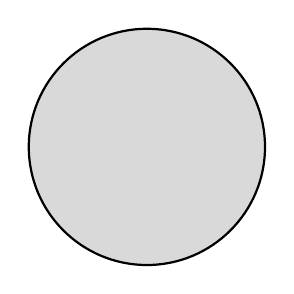
\begin{tikzpicture}[scale = 1.5]
            \filldraw[fill = black, fill opacity = 0.15, draw = black, thick] (0, 0) circle (1);
        \end{tikzpicture}
        \caption{Kružna membrana}
        \label{fig:membranes_circle}
    \end{subfigure}
    \begin{subfigure}{0.3\textwidth}
        \centering
        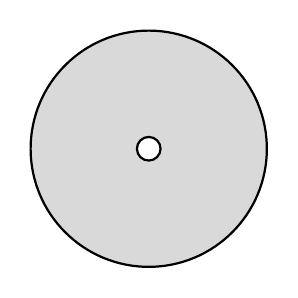
\begin{tikzpicture}[scale = 1.5]
            \scope
                \clip (-1.025, -1.025) rectangle (1.025, 1.025) (0, 0) circle (0.1);
                \fill[black, opacity = 0.15] (0, 0) circle (1);
            \endscope
            \draw[black, thick] (0, 0) circle (0.1);
            \draw[black, thick] (0, 0) circle (1);
        \end{tikzpicture}
        \caption{Membrana u obliku kružnog vijenca}
        \label{fig:membranes_annulus}
    \end{subfigure}
    \begin{subfigure}{0.3\textwidth}
        \centering
        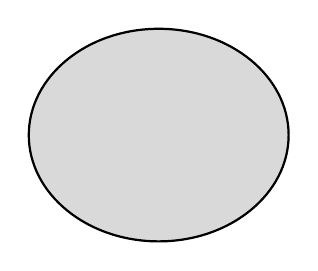
\begin{tikzpicture}[scale = 1.5]
            \filldraw[fill = black, fill opacity = 0.15, draw = black, thick] (0, 0) ellipse (1.1 and 0.9);
        \end{tikzpicture}
        \caption{Eliptična membrana}
        \label{fig:membranes_ellipse}
    \end{subfigure}
    \caption{Pojednostavljene ilustracije kružne membrane, membrane u obliku kružnog vijenca i eliptične membrane}
    \label{fig:membranes}
\end{figure}

\par

Konstrukcijom primjera bubnjeva iz prethodnog odlomka može se praktično provjeriti što znači da se dvije membrane (dva skupa u $ \reals^{\numprint{2}} $) \emph{malo} razlikuju. Na primjer, zamislimo bubanj čija membrana ima oblik kruga, bubanj čija membrana ima oblik kružnog vijenca tako da je vanjska kružnica jednakog radijusa kao radijus membrane prvog bubnja i bubanj čija je membrana eliptičnog oblika s obje poluosi \emph{gotovo jednake} kao radijus membrane prvog kruga (\seetxt~sliku~\ref{fig:membranes}). Koliko god unutarnja kružnica kao unutarnji rub membrane drugog bubnja bila mala ili čak radijusa $ \numprint{0} $, blizu središta koncentričnih kružnica membrana ne može \emph{slobodno} titrati jer na rubu membrane vrijednost svake svojstvene funkcije mora biti jednaka $ \numprint{0} $ (membrana je na rubu fiksno spojena s kućištem). S druge strane, na prvom bubnju središnja točka membrane može slobodno titrati, što će, uostalom, i činiti pri vibriranju po prvoj prirodnoj frekvenciji---u središtu je ekstrem svojstvene funkcije pridružene najnižoj svojstvenoj vrijednosti. No, treći i prvi bubanj vibrirali bi i zvučali \emph{slično}, to jest, spektri i svojstvene funkcije Laplaceovog operatora na takvom krugu i na takvoj elipsi tek bi se \emph{malo} razlikovali.

\par

Osim teorema~\ref{thm:Laplacian_eigenvalue_similar_domains} i \ref{thm:Laplace_eigenvalue_continuity}, još jedno obilježje svojstvenih vrijednosti skupova navode Fattah i Berrada u~\cite{bib:Fattah18}. Naime, ako je $ \Omega_{\numprint{1}} \subseteq \Omega_{\numprint{2}} $, onda je $ k $-ta najmanja svojstvena vrijednost skupa $ \Omega_{\numprint{1}} $ veća (ne nužno strogo) od $ k $-te najmanje svojstvene vrijednosti skupa $ \Omega_{\numprint{2}} $ za svaki $ k \in \positives{\naturals} $---drugim riječima, parcijalno preslikavanje iz teorema~\ref{thm:Laplace_eigenvalue_continuity} i padajuće je s obzirom na relaciju inkluzije. Iz teorema~\ref{thm:Laplacian_eigenvalue_similar_domains} i prethodno spomenutog sada je jasno da, što je domena veća, to su joj svojstvene vrijednosti manje. Oprimjereno proučavanjem stvarnog svijeta, među instrumentima obično su najdublji instrumenti u svakoj skupini instrumenata oni najveći---bubnjevi najdubljeg tona imaju najveće membrane, a kontrabasi imaju deblje i dulje žice od violine. Primjer nalazimo i u klaviru kao jedinstvenom instrumentu, gdje su žice dubljih tonova deblje i dulje od žica viših tonova.

\par

\begin{definition} \label{def:diameter}
    Neka je $ n \in \positives{\naturals} $. Neka je $ S \subseteq \reals^{n} $. \defined{Dijametar skupa $ S $}, označen s \defined{$ \diameter \left( S \right) $}, definiramo tako da vrijedi
    \begin{enumerate}
        \item ako je $ S = \emptyset $, onda je $ \diameter \left( S \right) = \numprint{0} $,
        \item ako $ \sup \left( \left\{ \distance{P}{Q} : P , Q \in S \right\} \right) $ po refleksivnom uređaju postoji i konačan je, onda je $ \diameter \left( S \right) $ jednak tom supremumu,
        \item inače je $ \diameter \left( S \right) = {+ \infty} $.
    \end{enumerate}
\end{definition}

\par

Uočimo da je $ \diameter \left( S \right) = \numprint{0} $ ako i samo ako je $ \card \left( S \right) \leq \numprint{1} $. Implikacija zdesna nalijevo očita je iz definicije~\ref{def:diameter}, a u suprotnom smjeru dokazujemo obratom po kontrapoziciji. Naime, ako postoje barem dvije različite točke u skupu $ S $, onda je njihova udaljenost strogo pozitivna pa supremum svih udaljenosti u skupu $ S $ ne može biti jednak $ \numprint{0} $. Iz ovoga lako slijedi da svaki neprazni otvoreni skup nužno ima dijametar različiti od $ \numprint{0} $.

\par

Također, dijametar je rastuć s obzirom na relaciju inkluzije. Udaljenost točaka je, po definiciji, nenegativna vrijednost, a po definiciji~\ref{def:diameter} dijametar skupa, osim supremuma skupa udaljenosti, može biti još i $ \numprint{0} $ ili pozitivna beskonačnost. Od svih je mogućih vrijednosti $ \numprint{0} $ najmanja vrijednost, što je ujedno i dijametar praznog skupa---najmanjeg skupa po relaciji inkluzije. Ako je, s druge strane, proizvoljni skup $ S $ neprazan, onda svaki nadskup skupa $ S $ sadrži sve točke koje sadrži i sam skup $ S $, stoga je i skup svih udaljenosti između točaka u skupu $ S $ podskup skupa svih udaljenosti između točaka u odabranom promatranom nadskupu. Rastuća monotonost sada proizlazi iz rastuće monotonosti supremuma ako dopuštamo da supremum može biti i beskonačan, a općenitost proizlazi iz proizvoljnosti skupa $ S $.

\par%
\clearpage%
\newpage

\begin{proposition} \label{prop:infinite_diameter}
    Neka je $ n \in \positives{\naturals} $ proizvoljan. Neka je $ S \subseteq \reals^{n} $ proizvoljan. Tada su sljedeće tvrdnje ekvivalentne:
    \begin{enumerate}
        \item \label{itm:infinite_diameter_unboundedness} skup $ S $ nije ograničen,
        \item \label{itm:infinite_diameter_arbitrary_distance} za svaki $ D > \numprint{0} $ postoje točke $ P , Q \in S $ takve da je $ \distance{P}{Q} \geq D $,
        \item \label{itm:infinite_diameter_infinite_diameter} dijametar skupa $ S $ je beskonačan.
    \end{enumerate}
\end{proposition}

\par

\begin{proof}
    Neka je $ n \in \positives{\naturals} $ proizvoljan. Neka je $ S \subseteq \reals^{n} $ proizvoljan.

    \par

    Dokazujemo sljedećim redom
    \begin{enumerate}
        \item Dokažimo da točka~\ref{itm:infinite_diameter_unboundedness} povlači točku~\ref{itm:infinite_diameter_infinite_diameter}.

            \par

            Pretpostavimo da skup $ S $ nije ograničen. Očito tada $ S $ nije prazan, pa možemo fiksirati neku točku $ P \in S $. Neka je $ D > \numprint{0} $ proizvoljan. Zbog neograničenosti skupa $ S $ postoji točka $ Q $ takva da je $ \norm{Q} \geq \norm{P} + D $. Po nejednakosti trokuta sada imamo
            \begin{equation*}
                \norm{P} + D \leq \norm{Q} = \distance{O}{Q} \leq \distance{O}{P} + \distance{P}{Q} = \norm{P} + \distance{P}{Q} \text{.}
            \end{equation*}
            Oduzimanjem $ \norm{P} $ iz gornje nejednakosti dobijemo $ \distance{P}{Q} \geq D $. Zbog proizvoljnosti $ D $ sada slijedi da skup $ \left\{ \distance{A}{B} : A , B \in S \right\} $ nema gornju među pa tako ni supremum kao najmanju gornju među. Drugim riječima, $ \diameter \left( S \right) = {+ \infty} $.

            \par

        \item Dokažimo da točka~\ref{itm:infinite_diameter_infinite_diameter} povlači točku~\ref{itm:infinite_diameter_arbitrary_distance}.

            \par

            Pretpostavimo da je dijametar skupa $ S $ beskonačan. Tada $ S $ nije prazan i ne postoji konačni supremum skupa $ \left\{ \distance{A}{B} : A , B \in S \right\} $ po refleksivnom uređaju. Zbog topološke potpunosti $ \reals $ to pak znači da taj skup nije ograničen odozgo, to jest, za svaki $ D > \numprint{0} $ postoje $ P , Q \in S $ takve da je $ \distance{P}{Q} \geq D $.

            \par

        \item Dokažimo da točka~\ref{itm:infinite_diameter_arbitrary_distance} povlači točku~\ref{itm:infinite_diameter_unboundedness}.

            \par

            Pretpostavimo da za svaku strogo pozitivnu vrijednost postoje točke u $ S $ koje su udaljene za barem toliko. Pretpostavimo i suprotno tvrdnji koju dokazujemo, to jest, da je $ S $ ograničen. Zbog ograničenosti skupa $ S $, postoji $ D > \numprint{0} $ takav da za svaku točku $ A \in S $ vrijedi $ \norm{A} < \frac{D}{\numprint{2}} $. No, tada za svake točke $ P , Q \in S $ po nejednakosti trokuta vrijedi
            \begin{equation*}
                \distance{P}{Q} \leq \distance{P}{O} + \distance{O}{Q} = \distance{O}{P} + \distance{O}{Q} = \norm{P} + \norm{Q} < \frac{D}{\numprint{2}} + \frac{D}{\numprint{2}} = D \text{.}
            \end{equation*}
            To je kontradikcija s početnom pretpostavkom, dakle, $ S $ nije ograničen.

            \par
    \end{enumerate}
\end{proof}

\par

\begin{proposition} \label{prop:finite_diameter}
    Neka je $ n \in \positives{\naturals} $ proizvoljan. Neka je $ S \subseteq \reals^{n} $ proizvoljan. Ako je $ S $ neprazan i ograničen, onda postoje točke $ P , Q \in \boundary S $ takve da vrijedi
    \begin{equation}
        \distance{P}{Q} = \diameter \left( S \right) \text{.}
    \end{equation}
\end{proposition}

\par

\begin{proof}
    Neka je $ n \in \positives{\naturals} $ proizvoljan. Neka je $ S \subseteq \reals^{n} $ proizvoljan. Pretpostavimo da je $ S $ neprazan i ograničen. Po obratu po kontrapoziciji iz propozicije~\ref{prop:infinite_diameter} tada slijedi da je dijametar skupa $ S $ konačan.

    \par

    Ako je $ S $ jednočlani skup, tvrdnja je trivijalna. Stoga pretpostavimo da $ S $ nije jednočlan.

    \par

    Ideja dokaza je sljedeća:
    \begin{enumerate}
        \item prikazati da za proizvoljne dvije točke u $ S $ postoje dvije točke na $ \boundary S $ koje su međusobno udaljenije (ne nužno strogo) od početne dvije točke,
        \item prikazati da se na $ \boundary S $ postiže maksimum udaljenosti dvije točke,
        \item prikazati da je maksimum udaljenosti dvije točke na $ \boundary S $ supremum udaljenosti dvije točke u $ S $.
    \end{enumerate}

    \par

    \begin{figure}[htb!]
        \centering
        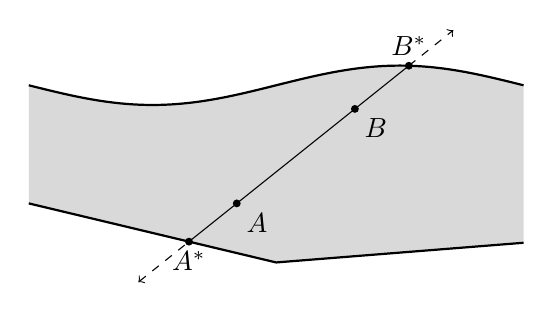
\begin{tikzpicture}
            % Skup.
            \fill[black, opacity = 0.15] (3.141592653589793, 1) sin (1.570796326794897, 1.25) cos (0, 1) sin (-1.570796326794897, 0.75) cos (-3.141592653589793, 1) -- (-3.141592653589793, -0.5) -- (0, -1.25) -- (3.141592653589793, -1) -- cycle;

            % Rub skupa.
            \draw[black, thick] (3.141592653589793, 1) sin (1.570796326794897, 1.25) cos (0, 1) sin (-1.570796326794897, 0.75) cos (-3.141592653589793, 1);
            \draw[black, thick] (-3.141592653589793, -0.5) -- (0, -1.25) -- (3.141592653589793, -1);

            % Pravac AB.
            \draw[black, thin, dashed, <-] (-1.75, -1.5) -- (-1.107118622461542, -0.985694897969234);
            \draw[black, thin] (-1.107118622461542, -0.985694897969234) -- (-0.5, -0.5);
            \draw[black, thin] (-0.5, -0.5) -- (1, 0.7);
            \draw[black, thin] (1, 0.7) -- (1.685448329892066, 1.248358663913653);
            \draw[black, thin, dashed, ->] (1.685448329892066, 1.248358663913653) -- (2.25, 1.7);

            % Tocke A^*, A, B, B^*.
            \fill[black] (-0.5, -0.5) circle (0.05) node[below right] {$ A $};
            \fill[black] (1, 0.7) circle (0.05) node[below right] {$ B $};
            \fill[black] (-1.107118622461542, -0.985694897969234) circle (0.05) node[below] {$ A^{{*}} $};
            \fill[black] (1.685448329892066, 1.248358663913653) circle (0.05) node[above] {$ B^{{*}} $};
        \end{tikzpicture}
        \caption[Pronalazak točaka na rubu skupa koje su udaljenije od točaka u skupu]{Pronalazak točaka na rubu skupa koje su udaljenije od točaka u skupu (u svrhu jednostavnosti skice izostavljen je koordinatni sustav). Na ovoj slici pravac \ensuremath{\straightline{A}{B}} siječe \ensuremath{\boundary S} samo dvaput, ali, naravno, moguće je da ga siječe i/ili dira i više puta---u tom slučaju točke \ensuremath{A^{{*}} , B^{{*}}} bile bi \emph{zadnja} sjecišta odnosno dirališta (nakon kojih u odgovarajućem smjeru pravac \ensuremath{\straightline{A}{B}} više nema zajedničkih točaka sa skupom \ensuremath{\closure{S}}).}
        \label{fig:finite_diameter_distant_points}
    \end{figure}

    \par

    Neka su $ A , B \in S $ proizvoljne različite točke. Promotrimo presjek pravca $ \straightline{A}{B} $ i skupa $ S $---pokazat ćemo da se na tom pravcu nalaze točke na $ \boundary S $ koje su međusobno udaljenije (ne nužno strogo) od točaka $ A $ i $ B $. Postupak koji slijedi ilustriran je na slici~\ref{fig:finite_diameter_distant_points}. Formalno, proučavat ćemo preslikavanja $ t \mapsto A + t \vectorline{A}{B} $ i $ t \mapsto B + t \vectorline{B}{A} $. Naime, zbog ograničenosti skupa $ S $ i zbog $ \vectorline{A}{B} , \vectorline{B}{A} \neq \Vec{\numprint{0}} $ (jer $ A \neq B $), slijedi da postoje $ T_{\numprint{1}} , T_{\numprint{2}} \in \reals $ takvi da za svaki $ t_{\numprint{1}} > T_{\numprint{1}} $ je $ B + t_{\numprint{1}} \vectorline{B}{A} \notin S $ i da za svaki $ t_{\numprint{2}} > T_{\numprint{2}} $ je $ A + t_{\numprint{2}} \vectorline{A}{B} \notin S $. Riječima, ako \emph{se} dovoljno \emph{pomaknemo} u jednom smjeru---orijentaciji, zapravo---po pravcu $ \straightline{A}{B} $, u jednom \emph{ćemo} trenutku \emph{izaći} iz skupa $ S $ i daljnjim kretanjem u toj orijentaciji više \emph{se} nikada \emph{ne ćemo vratiti} u skup $ S $. Kako je $ \reals $ topološki potpun, slijedi da supremumi
    \begin{align*}
        T_{\numprint{1}}^{{*}} & \coloneqq \sup \left( \left\{ t \in \reals : B + t \vectorline{B}{A} \in S \right\} \right) \text{,} \\
        T_{\numprint{2}}^{{*}} & \coloneqq \sup \left( \left\{ t \in \reals : A + t \vectorline{A}{B} \in S \right\} \right)
    \end{align*}
    po refleksivnom uređaju postoje. Oni su i veći (ne nužno strogo) od $ \numprint{1} $ jer su $ A = B + \vectorline{B}{A} , B = A + \vectorline{A}{B} \in S $. Označimo li
    \begin{align*}
        A^{{*}} & \coloneqq B + T_{\numprint{1}}^{{*}} \vectorline{B}{A} \text{,} \\
        B^{{*}} & \coloneqq A + T_{\numprint{2}}^{{*}} \vectorline{A}{B} \text{,}
    \end{align*}
    zaključujemo da za svaki $ \varepsilon > \numprint{0} $ u skupovima $ \openball{A^{{*}}}{\varepsilon} , \openball{B^{{*}}}{\varepsilon} $ postoje točke iz $ S $ i $ S^{\complement} $---vrijedi $ A^{{*}} , B^{{*}} \in \boundary S $. Također, budući da sve točke $ A^{{*}} , A , B , B^{{*}} $ pripadaju istom pravcu i to redom kojim su navedene (zbog načina konstrukcije točaka $ A^{{*}} , B^{{*}} $), vrijedi i
    \begin{equation*}
        \distance{A^{{*}}}{B^{{*}}} = \distance{A^{{*}}}{A} + \distance{A}{B} + \distance{B}{B^{{*}}} \geq \distance{A}{B} \text{.}
    \end{equation*}
    Zbog proizvoljnosti točaka $ A , B \in S $ slijedi da za izbor svake dvije točke u $ S $ postoje dvije točke na $ \boundary S $ koje su međusobno udaljenije od početne dvije točke (iako smo zadali ograničenje $ A \neq B $, ali za točke $ A = B $ njihova je udaljenost ionako najmanja moguća).

    \par

    Nadalje, kako je $ S $ ograničen, i $ \boundary S $ je ograničen pa je $ \boundary S $ kompaktni skup. Po Weierstrass-Bolzanovom teoremu zbog neprekidnosti udaljenosti slijedi da postoje $ P , Q \in \boundary S $ na kojima se postiže
    \begin{equation*}
        \distance{P}{Q} = \max \left( \left\{ \distance{X}{Y} : X , Y \in \boundary S \right\} \right) \text{.}
    \end{equation*}

    \par

    Za $ P , Q \in \boundary S $ iz prethodnog odlomka, budući da je rub skupa podskup skupa njegovih gomilišta, postoje nizovi $ \left( P_{i} \right)_{i \in \naturals} , \left( Q_{i} \right)_{i \in \naturals} $ u $ S $ koji konvergiraju k $ P , Q $ respektivno. Ponovo, zbog neprekidnosti udaljenosti slijedi da niz $ \left( \distance{P_{i}}{Q_{i}} \right)_{i \in \naturals} $ konvergira k $ \distance{P}{Q} $.

    \par

    Sve dokazano zapravo znači da su svake dvije točke u $ S $ udaljene za manje (ne nužno strogo) od $ \distance{P}{Q} $, ali i da postoji niz parova točaka u $ S $ kojima udaljenosti teže k $ \distance{P}{Q} $. Drugim riječima, $ \distance{P}{Q} $ je neka gornja ograda udaljenosti točaka u $ S $, ali i svaka gornja ograda udaljenosti točaka u $ S $ mora biti barem tolika---$ \distance{P}{Q} $ je supremum udaljenosti točaka u $ S $, to jest, dijametar skupa $ S $.
\end{proof}

\par

Iz propozicije~\ref{prop:finite_diameter} zapravo je jasno zašto je pojam iz definicije~\ref{def:diameter} nazvan \emph{dijametrom}. Uistinu, stvarni dijametar (dvostruki radijus) kružnice ili kruga jednak je dijametru kao vrijednosti pridruženoj skupu definiranoj u definiciji~\ref{def:diameter} jer nijedne dvije točke na kružnici nisu udaljene za strogo više od dvostrukog radijusa, a samo su točke na kružnici koje razapinju dužinu s polovištem u središtu kružnice udaljene za točno toliko.

\par

Po definiciji izometrije, primjena izometrije na skup \emph{čuva} skup udaljenosti točaka u skupu. Time je, u slučaju neprazog skupa, supremum---konačan ili beskonačan---udaljenosti točaka u skupu jednak u početnom i rezultantnom skupu, pa izometrične transformacije skupova \emph{čuvaju} dijametar skupa.

\par

Što se tiče skaliranja skupa, primijetimo prvo da za svaki neprazni skup $ S \subseteq \reals^{n} $ vrijedi $ \numprint{0} S = \left\{ O \right\} $, gdje je $ O $ ishodište prostora $ \reals^{n} $, bio $ S $ ograničen ili ne. Nadalje, za proizvoljne točke $ P , Q \in \reals^{n} $ i proizvoljni skalar $ \alpha \geq \numprint{0} $ raspisom standardne euklidske udaljenosti kao izraza ovisnog o koordinatama točaka dobije se da je $ \distance{\alpha P}{\alpha Q} = \alpha \distance{P}{Q} $, iz čega slijedi da je skup udaljenosti skaliranih točaka jednak skupu skaliranih udaljenosti. Ako skup udaljenosti, dakle, nije ograničen, skaliranjem nekom vrijednosti različitom od $ \numprint{0} $, on ponovo ostaje neograničen, a, ako je ograničen, supremum skaliranog skupa jednak je skaliranom supremumu originalnog skupa. Prethodnim i ovim odlomkom dokazana je sljedeća propozicija.

\par

\begin{proposition} \label{prop:diameter_similar_sets}
    Neka je $ n \in \positives{\naturals} $ proizvoljan. Neka su $ S , T \subseteq \reals^{n} $ proizvoljni. Ako je $ S \sim T $ i ako je $ \alpha \varphi \colon \reals^{n} \to \reals^{n} $ sličnost skupa $ T $ sa skupom $ S $ za neku izometriju $ \varphi \colon \reals^{n} \to \reals^{n} $ i neki skalar $ \alpha > \numprint{0} $, onda je
    \begin{equation}
        \diameter \left( T \right) =
        \begin{cases}
            \alpha \diameter \left( S \right) & \diameter \left( S \right) \ \text{konačan} \text{,} \\
            {+ \infty} & \text{inače}
        \end{cases}
        \text{.}
    \end{equation}
\end{proposition}

\par

Neke posljedice propozicije~\ref{prop:diameter_similar_sets} su sljedeće:
\begin{enumerate}
    \item \label{itm:similarity_zero_diameter} skup dijametra $ \numprint{0} $ i skup dijametra različitog od $ \numprint{0} $ ne mogu biti slični,
    \item \label{itm:similarity_infinite_diameter} skup konačnog dijametra i skup beskonačnog dijametra ne mogu biti slični,
    \item \label{itm:similarity_finite_diameter_equality} za svaki skup konačnog dijametra različitog od $ \numprint{0} $ postoji skup dijametra $ \numprint{1} $ koji mu je sličan (proizvoljni skup $ S $ možemo, na primjer, skalirati s $ \diameter^{{- \numprint{1}}} \left( S \right) $ ako je $ 0 < \diameter \left( S \right) < {+ \infty} $),
    \item ako su dva skupa slična i imaju konačni i međusobno jednaki dijametar, onda su oni isti do na izometrične transformacije,
    \item \label{itm:similarity_finite_diameter_transformation} točke na rubu nepraznog skupa s konačnim dijametrom čija je udaljenost jednaka dijametru tog skupa preko sličnosti se preslikavaju u točke na rubu nekog drugog skupa (koji je sličan onom početnom skupu) čija je udaljenost jednaka dijametru tog drugog skupa (\seetxt~propoziciju~\ref{prop:finite_diameter}).
\end{enumerate}

\par

\begin{corollary} \label{cor:spectrum_similar_domains}
    Neka je $ n \in \positives{\naturals} $ proizvoljan. Neka su $ \Omega_{\numprint{1}} , \Omega_{\numprint{2}} \subseteq \reals^{n} $, $ \Omega_{\numprint{1}} , \Omega_{\numprint{2}} \neq \emptyset $, proizvoljni ograničeni i otvoreni takvi da su $ \boundary \Omega_{\numprint{1}} , \boundary \Omega_{\numprint{2}} $ po dijelovima glatki. Ako je $ \Omega_{\numprint{1}} \sim \Omega_{\numprint{2}} $, onda je
    \begin{equation}
        \diameter^{\numprint{2}} \left( \Omega_{\numprint{1}} \right) \spectrum \left( \Omega_{\numprint{1}} \right) = \diameter^{\numprint{2}} \left( \Omega_{\numprint{2}} \right) \spectrum \left( \Omega_{\numprint{2}} \right) \text{.}
    \end{equation}
\end{corollary}

\par

\begin{proof}
    Ovo je zapravo direktna posljedica propozicije~\ref{prop:diameter_similar_sets} i teorema~\ref{thm:Laplacian_eigenvalue_similar_domains} kada uzmemo u obzir da su zbog nepraznosti i otvorenosti domena njihovi dijametri nužno strogo pozitivni, a po obratu po kontrapoziciji propozicije~\ref{prop:infinite_diameter} dijametri domena nužno su i konačni.
\end{proof}

\par

Rezimirajmo sada dosadašnje rezultate koji pojednostavljuju računanje spektra skupa:
\begin{enumerate}
    \item \label{itm:spectrum_domain_normalisation} Spektri sličnih skupova razlikuju se samo skaliranjem za kvadrat omjera dijametara---ako je poznat spektar skupa sličnog skupu od interesa i ako je poznat omjer dijametara tih skupova, spektar skupa od interesa lako se izračuna. Normalizacija domene prvenstveno će se odnositi na traženje slične domene dijametra $ \numprint{1} $ jer je tada omjer dijametara trivijalan.
    \item \label{itm:spectrum_approximation} Ako su oblici (uzimajući u obzir i njihovu veličinu) dva skupa \emph{gotovo jednaki}, spektri im se \emph{malo razlikuju}---dodatno, zbog monotonosti spektra na svakom indeksu tada je moguće spektar nekog skupa aproksimirati kao nekakvu sredinu (na primjer, aritmetičku) spektra jednog njegova podskupa i jednog njegova nadskupa koji se oblikom i veličinom ne razlikuju \emph{mnogo}. Spomenuti postupak jedan je način kako se spektar \emph{kompliciranije} domene može aproksimirati. Osim aproksimacije \emph{s obje strane}, moguće je naprosto računati spektar nekog skupa \emph{gotovo jednakog} oblika kao početni skup.
    \item \label{itm:diameter_computation} Za pronalazak dijametra skupa dovoljno je maksimizirati udaljenost točaka na njegovu rubu---u specijalnim slučajevima u kojima je rub skupa određena vrsta krivulje uz dovoljno (i to konačno mnogo) informacija ta se vrijednost može jednostavno izračunati (na primjer, \seetxt~propoziciju~\ref{prop:diameter_polygon}).
\end{enumerate}
Naravno, kada se u prethodnim točkama spominje spektar skupa, specijalno te tvrdnje vrijede i ako se promatraju samo \emph{izabrani} indeksi spektra (najčešće prvih nekoliko konačno mnogo indeksa).

\par

Zbog točke~\ref{itm:spectrum_approximation} iz prethodnog odlomka u ostatku rada bavit ćemo se samo poligonima. Poligonima svakako nije moguće aproksimirati proizvoljne skupove koji zadovoljavaju uvjete iz definicije~\ref{def:Laplacian_eigen} (na primjer, skupovi s \emph{rupama} kao na slici~\ref{fig:membranes_annulus}), ali ograničeni skupovi čiji su rubovi po dijelovima glatke jednostavne zatvorene krivulje mogu se aproksimirati poligonima.

\par
